On this section, we discuss about the solution developed, starting from the data structure, which the work relies, then the algorithms used to do the grouping mechanism, then the cluster algorithm and the overall methodology. \\

  The methodology can be summarized in the following process:\\
  First, we trace a program using statically or dynamically embedded tracepoints. Then we read the tracing and develop a CCT recording, also the performance metrics. Later, we run the clustering techniques and the association rule, which indicated the possible cause of the performance issue.
  
    \subsubsection{Recording of execution}
    We record the program executing using LTTng, this tracer has low overhead, therefore is adequate for this type of research. 
    The trace is also recorded with the performance metrics such as instructions, cache-misses, page-faults, and schedule switches by using the perf counters tools in Linux.
    
    \subsubsection{Generating the data structure}
    After the recording in different scenarios, a pre-processing of building a structure for comparison is done, this structure is a enhanced calling context tree. 
    To do this process, we use trace compare to divide the tracing in segments, delimited using: e.g. in the case of sys\_open, we used systemCallOpen and systemCallExit.
    In this process we aim to construct comparable information using ECCT (or EDT), which each node represent a call and the information in this call will be within the nodes. A delta of the entry and the exit for each metric is recorded in the node, in a sampling scheme.
    
    \subsubsection{Clustering technique}
    After the data was pre-processed and the tree is built, a mathematical model is done and its behaviour compared to its input can be determined. 
    
    \subsubsection{Execution Comparison}
    With the groups divided the next phase is the comparison among them. There are possible to ways to compare the groups: compare the mean and median for each group or use the Apriori Association described in section \ref{sec:association}.
    
\subsection{Data Structure}
% \textit{Call Graph}\\
%     The call graph is a useful data representation for control and data flow programs which investigate interprocedural communication (i.e., how procedures exchange information). It contains all the relationships among the procedures in a program and can contain auxiliary information concerning the
%     data within each procedure and global data shared among procedures \cite{call_graph}.

\textit{Calling Context Tree}\\
Calling contexts are very important for a wide range of applications such as profiling, debugging, and event logging. Most applications perform expensive \textit{stack walking} to recover contexts\cite{precise}. The resulting contexts are often explicitly represented as a sequence of call sites and hence bulky. The goal of calling context encoding is to uniquely represent the current context of any execution point using a small number of integer identifiers (IDs). This data structure was introduced by \cite{27} and reused by \cite{4}, \cite{28}.
% \textit{Enhanced Calling Context Tree}\\
    In this work we aggregate data, related to the performance on the Calling Context Tree, which gives the concept of enhanced structure. The aggregated data is related with the performance metrics, the data is added in the tree nodes and gives the possibility to be analyzed off-line.
    The Figure \ref{fig:ecct_dt} demonstrates the difference between the dynamic tree and the calling context tree.
    \begin{figure}[h]
        \centering
        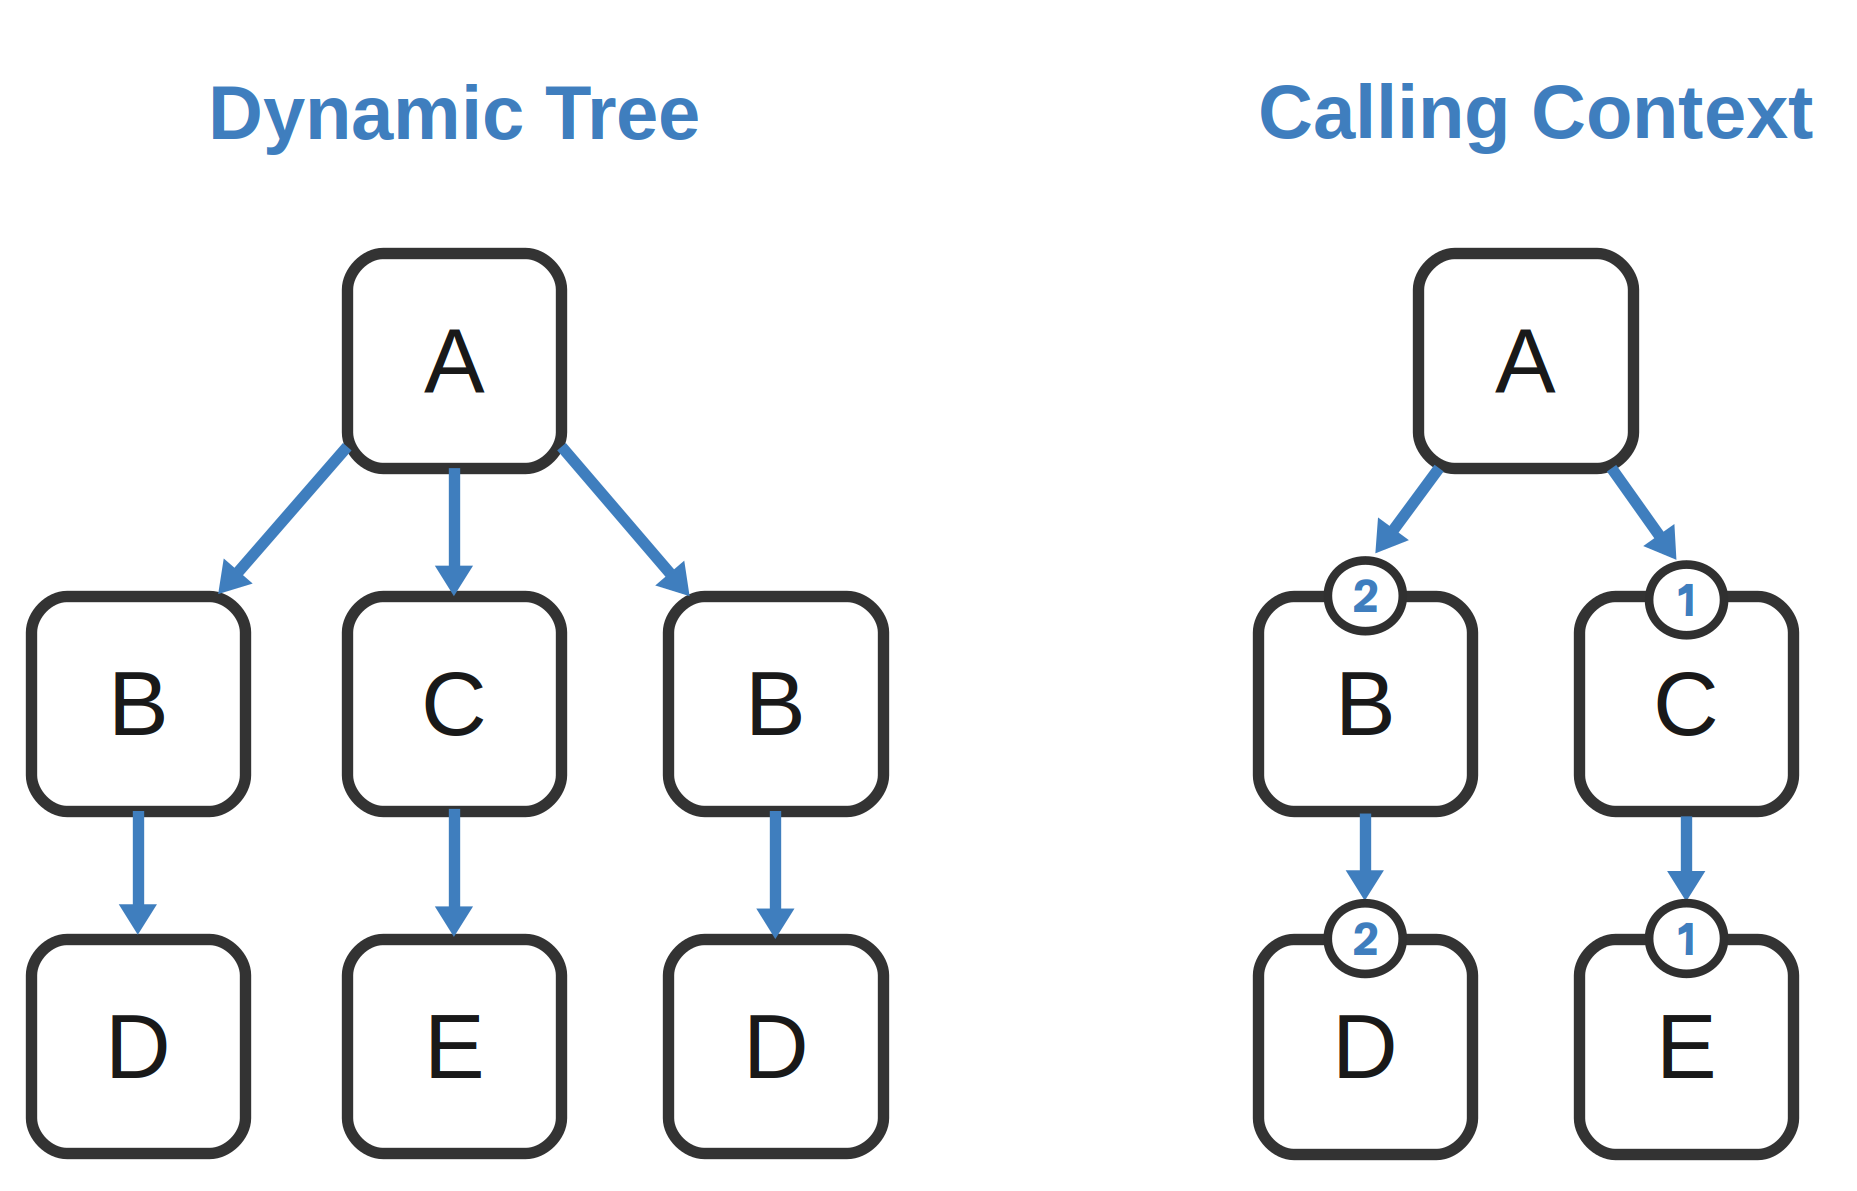
\includegraphics[width=0.40\textwidth]{figures/dynamic-calling.png}
        \caption{Dynamic Call Graph vs Enhanced Calling Context Tree }
        \label{fig:ecct_dt}
    \end{figure}
    The metrics recorded inside the tree are described in the subsection Performance Metrics.
    
\textit{Performance Metrics}\\
    In virtue of generating a tree through a tracing approach, it is possible to record runtime information of the system \cite{francis1}.
    They are recorded using the lttng feature add-context, and this gives the possibility to add performance counters in the tracing session.\\
    Example: perf:cache-misses, perf:major-faults, perf:branch-load-misses\\
    This technique was explored in the work of \cite{doray_thesis} and \cite{olsa}.
    Although we took several metrics in consideration, we summarizes three metrics before introduce the clustering mechanism.\\
    
%\textbf{cache-misses}\\ 
%       When a program accesses a memory location that is not in the cache, it is called a cache miss. Since the processor has to wait for the data to be fetched from the next cache level or from main memory before it can continue to execute, cache misses directly influence the performance of the application \cite{washington}.
%       The concept of cache miss ratio, is the ratio of memory accesses that cause a cache miss. From the miss ratio you can usually tell whether cache misses may be a performance problem in an application.
      
%\textbf{page-faults}\\
%       A page fault is the sequence of events occurring when a program attempts to access data (or code) that is in its address space, but is not currently located in the system's RAM. The operating system must handle page faults by somehow making the accessed data memory resident, allowing the program to continue operation as if the page fault had never occurred\cite{redhat}.
      
%\textbf{cpu instructions}\\ 
%       This metric is the measurement of the instructions related to arithmetic, logical and shift operations on values in registers. 
    
    
\subsection{Data Structure Construction}
    The construction of the ECCT involves the reading of the tracing in order and simultaneously building the nodes as soon as the data is coming. It is necessary to delimit the boundaries of the nodes in the tree. Therefore, to set events as starting and end points of the nodes. Depending on the case, the construction of the tree depending on the case might be easy to be done using a ECT, instead of ECCT.\\
    Consequently, it is necessary to demultiplex the events on the trace. To do so, the trace must provide a way to identify the start and end points of each execution. 
    For this process there are two approaches:\\
    First, use existing events of the Linux kernel. As an example, the syscall\_exit\_accept event (generated when a connection is accepted on a socket) and the syscall\_entry\_shutdown event (generated when a connection is closed) correctly delimit requests received by an Apache server. \\
    Second, is to use LTTng-UST probes, statically inserted in the source code. Different probe types can be used to delimit different execution types. In that way, the delimitation of the nodes can be done.
    An advantage the first approach is to use existing events and thus, no access to the source code is required. The advantages of the second is that no kernel knowledge is required to use this process.
    
    The Figure \ref{fig:ecct_build}, demonstrates the mechanism used to create the ECCT from the tracing file.
    
\begin{figure}[h]
      \centering
        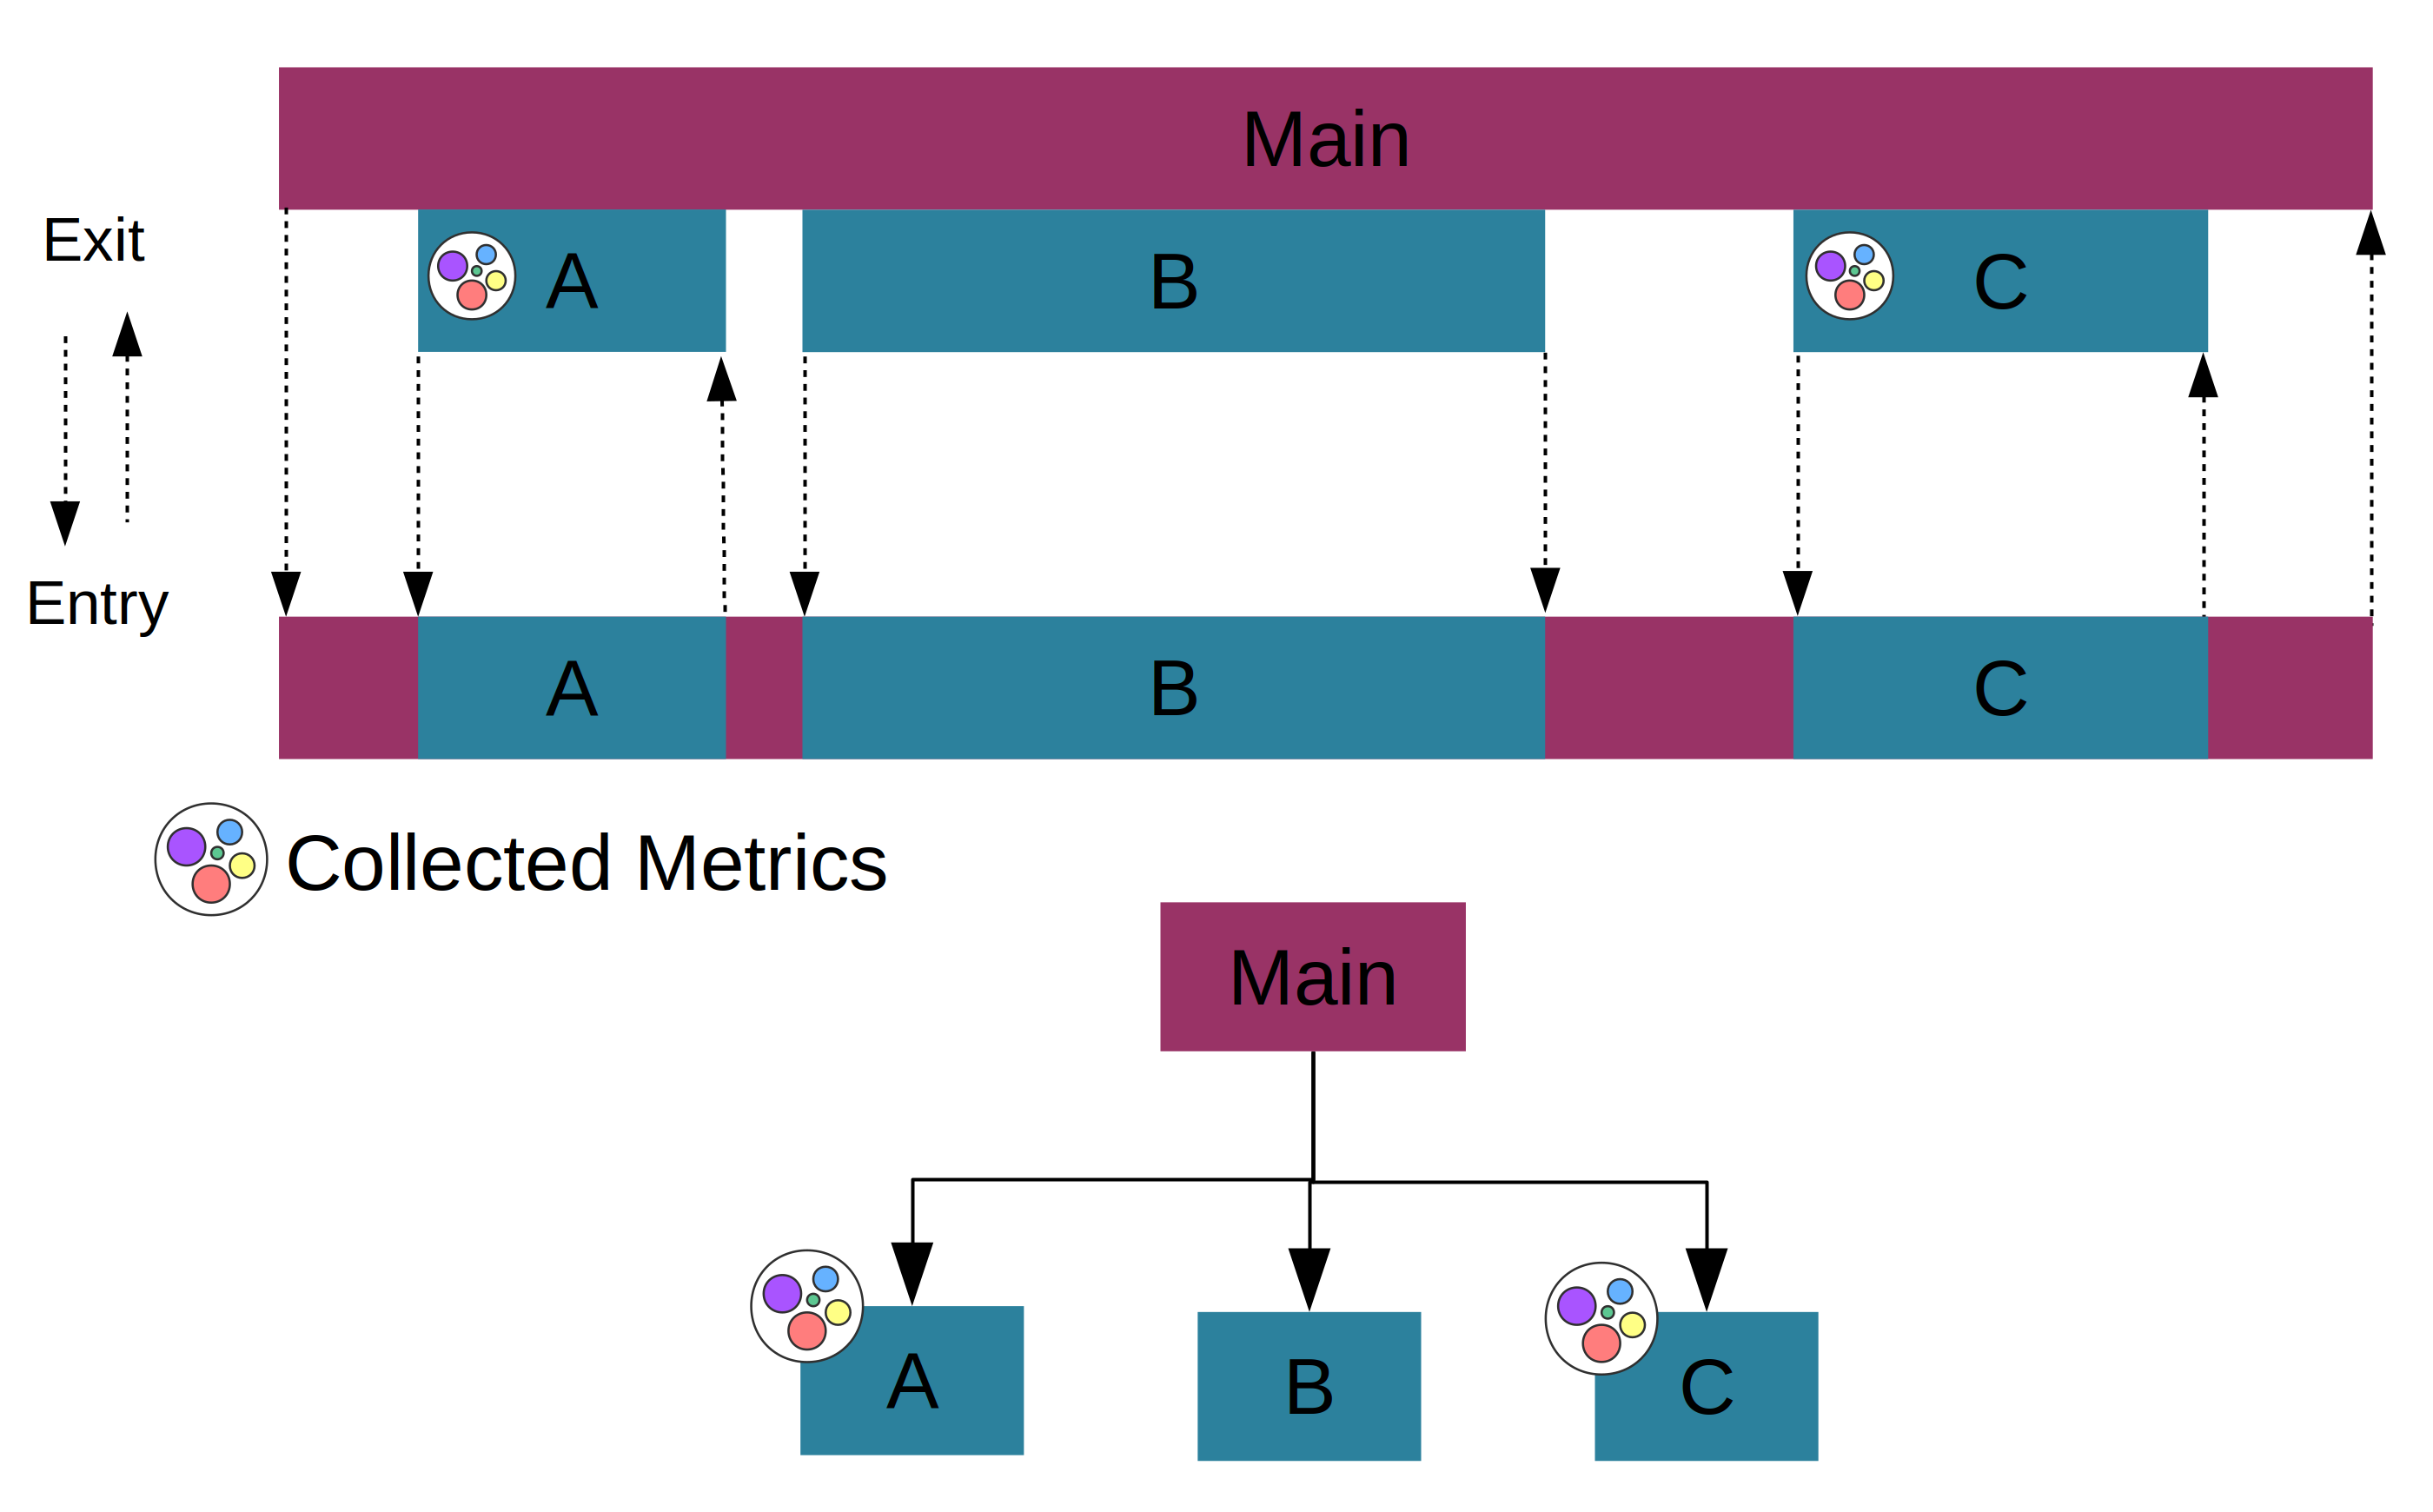
\includegraphics[width=0.50\textwidth]{figures/ecct.png}
        \caption{Enhanced Calling Context}
        \label{fig:ecct_build}
    \end{figure}
    
    After the construction of the tree the clustering mechanisms, described below, can be applied.\\
  
\subsection{Clustering}
\label{sec:clustering}
On this part we outline the clustering techniques used for the metrics grouping, the heuristic to do an automated classification mechanisms and finally the association rule used to find the metric which impacted on the performance of the executions.\\

% \textbf{Clustering techniques}
% \textit{ Supervised and non-supervised machine learn methods}\\
%     Supervised learning is the machine learning task of inferring a function from labeled training data. The training data consist of a set of training examples. In supervised learning, each example is a pair consisting of an input object (typically a vector) and a desired output value (also called the supervisory signal). A supervised learning algorithm analyzes the training data and produces an inferred function, which can be used for mapping new examples. 
    
%     Unsupervised machine learning is the machine learning task of inferring a function to describe hidden structure from "unlabeled" data (a classification or categorization is not included in the observations). Since the examples given to the learner are unlabeled, there is no objective evaluation of the accuracy of the structure that is output by the relevant algorithm—which is one way of distinguishing unsupervised learning from supervised learning and reinforcement learning.
    
\textit{Support Vector Machines}\\
In machine learning, support vector machines are supervised learning models with associated learning algorithms that analyze data used for classification and regression analysis. Given a set of training examples, each marked as belonging to one or the other of two categories, an SVM training algorithm builds a model that assigns new examples to one category or the other, making it a non-probabilistic binary linear classifier. 
Besides teaching the model, the restriction is another drawback of using SVMs. The major drawback of this model is the division in two groups, so relevant information could be lost and no further comparison technique could be applied later.

    
% \textit{Mean Swift}\\
%     MeanShift clustering aims to discover blobs in a smooth density of samples. It is a centroid based algorithm, which works by updating candidates for centroids to be the mean of the points within a given region. These candidates are then filtered in a post-processing stage to eliminate near-duplicates to form the final set of centroids.
%     Given a candidate centroid x i for iteration t, the candidate is updated according to the following equation:
    
%     %x_i^{t+1} = x_i^t + m(x_i^t)
    
%     Where N(xi) is the neighborhood of samples within a given distance around xi and m is the mean shift vector that is computed for each centroid that points towards a region of the maximum increase in the density of points. This is computed using the following equation, effectively updating a centroid to be the mean of the samples within its neighborhood:
%     %m(x_i) = \frac{\sum_{x_j \in N(x_i)}K(x_j - x_i)x_j}{\sum_{x_j \in N(x_i)}K(x_j - x_i)}
    
%     The algorithm automatically sets the number of clusters, instead of relying on a parameter bandwidth, which dictates the size of the region to search through. This parameter can be set manually, but can be estimated using the provided estimate bandwidth function, which is called if the bandwidth is not set.
%     The algorithm is not highly scalable, as it requires multiple nearest neighbor searches during the execution of the algorithm. The algorithm is guaranteed to converge, however the algorithm will stop iterating when the change in centroids is small \cite{mean_swift}.

\textit{Percentage classification}\\
The percentage classification was done by comparing the metrics and separate them by a percentage threshold, which is the mean of the group. The percentage classification is interesting considering sometimes that the distribution is not so spaced to create clusters. The naive classification will draw a group even when they are too close and would be in just one group for other clustering techniques.
    
\textit{K-means}\\
K-means is a simple unsupervised machine learning algorithm that groups a dataset into a user-specified number (k) of clusters. The algorithm is somewhat naive it clusters the data into k clusters, even if k is not the right number of clusters to use. Therefore, when using k-means clustering, users need some way to determine whether they are using the right number of clusters.
Since, the number of groups must be known before applying the k-means, another technique needs to be applied in order to find the appropriate number of groups (k). 
    
    
\textit{Comparing Models}\\
Comparing the three techniques described above, the conclusions were. First, the SVM model was able to delimit the difference between the slow executions and fast executions. However, the delimitation is in just two groups. \\
The second mechanism, Percentage classification, is a unsupervised mechanism and leads to segregation of data even if they are homogeneously distributed among the dataset. \\
Finally the k-means algorithm is efficient but requires the number of groups to be used in the classification process. Comparing the models we developed the technique to use an heuristic classification to make the clustering process automatic.
    
    
\textit{Auto Clustering}\\
Considering the models shown above, we chose to develop a non-supervised method, called auto clustering. The possibility to use an automated approach is more interesting for us in comparison with a non-automated methods, mainly because we aim not to use the data to train the model. Therefore we implemented a version of comparative k-means using the SSE (sum of square errors) variability information, plus an heuristic evaluation. This technique can be used for an arbitrary dimension of since the amount of difference, SSE (sum of squared error), can be calculated on those cases \cite{multi_dimentionals_sse}.
    
\subsection{\textbf{Automatic Clustering through heuristic Evaluation}}

    \textit{Elbow method}\\
    One method to quantitatively measure the number of clusters is the elbow method. This method compares the sum of squared errors (SSE) considering several numbers of groups from the classification used. 
    The elbow method gives the possibility to use the SSE to find the elbow value, which can be defined as a value which the SSE changes its behaviour abruptly. In our cases, the elbow value is when the SSE stop decreasing substantially.
    
    However, the elbow method does not guarantee a perfect match in cases which the data is well distributed. Instead, the analysis of the SSE can give a smooth curve and the best value for number of groups is not precisely defined. In cases like this, we developed another clustering based on the mean distance of the data.
    %try a different method for determining the optimal k, such as computing silhouette scores, or we might reevaluate whether clustering is the right thing to do on our data.
    
    \textit{Heuristic Evaluation}\\
    To compare the SSE values, we needed also to do an heuristic function which compares the different values of the SSE to compute the Elbow. 
    Therefore, we use this approach to compare several runs of classifications and extract the one with less squared errors. The used heuristic is to take as optimal group the biggest gap on an array of SSE values. 
    
    The Figure \ref{fig:sse}, shows an illustration of the SSE and the elbow value. The elbow value is the number that marks the change on the path of the function, in the example is number of groups 2.
    
    \begin{figure}[h]
      \centering
        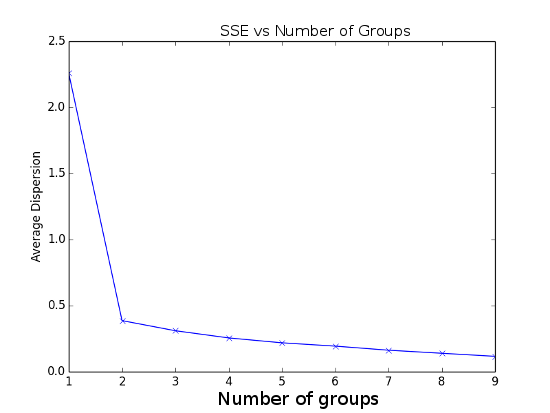
\includegraphics[width=0.50\textwidth]{figures/SSE.png}
        \caption{Elbow method: SSE Comparison}
        \label{fig:sse}
    \end{figure}


\subsection{\textbf{Association among the Groups}}
\label{sec:association}
The clustering of metrics is just a part of the approach, since a rule of groups need to be applied to find the specific cause for the discrepancy on the executions. To solve this problem and find the cause of the difference, after the grouping mechanism we applied a set association rule. Therefore, using a set exclusion, we can find the metric that is responsible for the elapsed time.
The association rule is illustrated on the Figure \ref{fig:association}, which describes a metric X and the elapsed time comparison. The grouping on the Metric x divides the data in two groups and those groups are the intrinsic related to the elapsed time group. \\
The association rule can be applied in an arbitrary classification algorithm with several different dimensions, so the association can be defined as a heuristic to find root cause problems using grouping or clustering algorithms.

A matrix of groups correlation can be done to better understand the relation among the groups.


    % \begin{figure}[h]
    %   \centering
    %     \includegraphics[width=0.50\textwidth]{figures/association.png}
    %     \caption{Association of groups through Apriori algorithm}
    %     \label{fig:association}
    % \end{figure}
    
\begin{table}[h]
\centering
\begin{tabular}{cccc}
                      & A                         & B                        & C     \\ \hline
                      &                           &                          &       \\ 
A                     & X                         & 75\%                     & 100\% \\ \hline
                      &                           &                          &       \\ 
B                     & 75\%                      & X                        & 65\%  \\ \hline
                      &                           &                          &       \\
\multicolumn{1}{l}{C} & \multicolumn{1}{l}{100\%} & \multicolumn{1}{l}{65\%} & X     \\ \hline
\end{tabular}
\vspace{10pt}
\caption{Association of groups through Apriori algorithm}
\label{fig:association}
\end{table}

\subsection{\textbf{Accuracy of the model}}
The association will give the group of metrics that are related with slow and fast runs, however, there is the possibility of false positives and false negatives. The accuracy of the model is related with the size of the groups given, i.e. the all slow executions will be in one group, however the related metric, which explains the reason, is bigger than the associated group.  In summary, if the groups overlap, main metric and slow executions, no false positives of negatives were found, even though the overlap does not mean is responsible for the performance problem, it is only an indication factor. In this matter, statistics is an indicator of underlying causes, which requires some complementary analysis to be confirmed.
    
    
\section{Solution Implementation}
\label{sec:implementaion}
\begin{figure*}[t!]
  \centering
    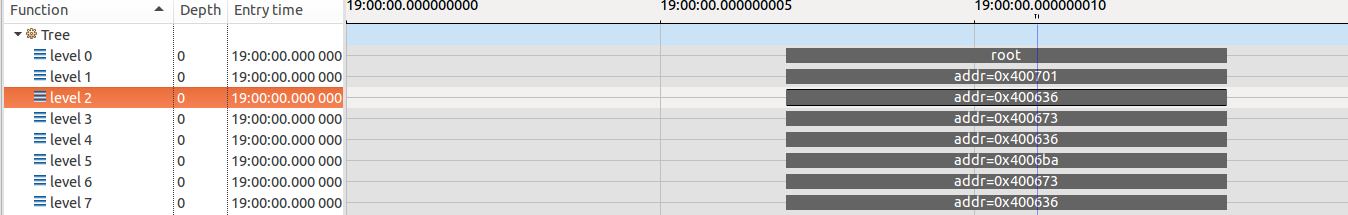
\includegraphics[width=1.0\columnwidth]{figures/cct_view.png}
    \caption{CCT View in TraceCompass }
    \label{fig:cct_view}
    \vspace{-10pt}
\end{figure*}

We describe on this section the implementation of the Calling Context Tree in TraceCompass, the Flame Graph comparison, and the Auto cluster mechanism.

The CCT View is an analysis developed in TraceCompass framework \cite{tracecompass}, which specifically aims to study the CCT and its variations. The module with Auto clustering was included on it. The view displays the calling functions in a graphic view that helps the developer/tester to improve their codes and to compare the traces using the approach described on this work.\\

\textbf{\textit{Tree Construction}}\\
The CCT View builds the tree from the tracing as explained in the section Tree Construction. In summary the tracing is read in order and event entry-exit pairs are grouped in nodes, sub-nodes are defined by pairs of entry-exit inside the above node. The data found, i.e the performance metrics, of the nodes is summarized for the respective node. The tree is build to summarized the redundant nodes, thus, avoiding the build of a Dynamic Call Tree. Figure \ref{fig:cct_view}, shows this feature in the CCT View.\\

\textbf{\textit{Differential Flame Graph}}\\
The CCT View implements a Differential Flame Graph view to compare executions and groups of executions. Usually the Differential Flame Graph compares two executions, but on our implementation it is possible to compare groups of executions. In our implementation the flame graphs are composed of three colors: green (to represent equals amount of time), red (slower executions) and gray (faster executions). 

Figure \ref{fig:flame}, shows a diagram of the RGG Differential Flame Graph, the green color shows the functions which are faster in the main execution, the grey part means they are equal and the red part means that this function is slower with the comparative one. The name, RGG flamegraph brings allusion of this concept in contrast with Brendan Gregg's Red/Blue Flame Graph. 
 
 \begin{figure}[h]
  \centering
    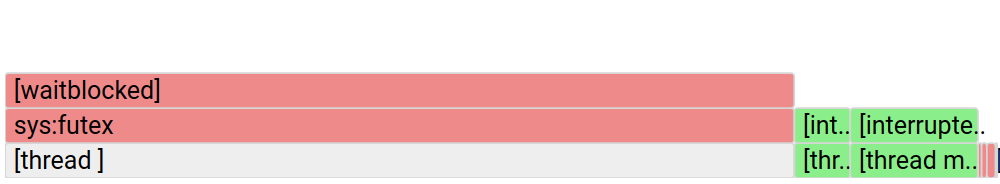
\includegraphics[width=1.0\textwidth]{figures/framegraph.png}
  \caption{RGG Differential Flame Graph Diagram}
  \label{fig:flame}
\end{figure}

\textbf{\textit{Auto cluster}}\\
The Auto cluster feature was implemented on CCTView to help developers execute similar performance cause analysis on tracing. The heuristic evaluation (elbow method) and the clustering techniques (k-means and percentage clustering) were implemented separately, therefore the developer can choose the most suitable one.\\
    
\textbf{\textit{Correlation feature}}\\
Another feature of the CCT View is the possibility to find the correlation matrix of the metrics. 
As the dictum states, \textit{correlation does not imply causation}, which means that correlation by itself cannot be used to infer a causal relationship between the studied variables.
        
    